\documentclass[11pt]{aghdpl}
% \documentclass[en,11pt]{aghdpl}  % praca w języku angielskim

% Lista wszystkich języków stanowiących języki pozycji bibliograficznych użytych w pracy.
% (Zgodnie z zasadami tworzenia bibliografii każda pozycja powinna zostać utworzona zgodnie z zasadami języka, w którym dana publikacja została napisana.)
\usepackage[english,polish]{babel}

% Użyj polskiego łamania wyrazów (zamiast domyślnego angielskiego).
\usepackage{polski}

\usepackage[utf8]{inputenc}

% dodatkowe pakiety

\usepackage{mathtools}
\usepackage{amsfonts}
\usepackage{amsmath}
\usepackage{amsthm}
\usepackage{multirow}
\usepackage{url}
%\usepackage{iopams}

% --- < bibliografia > ---

%\usepackage[
%style=numeric,
%sorting=none,
%%
%% Zastosuj styl wpisu bibliograficznego właściwy językowi publikacji.
%language=autobib,
%autolang=other,
%% Zapisuj datę dostępu do strony WWW w formacie RRRR-MM-DD.
%%urldate=iso8601,
%% Nie dodawaj numerów stron, na których występuje cytowanie.
%backref=false,
%% Podawaj ISBN.
%isbn=true,
%% Nie podawaj URL-i, o ile nie jest to konieczne.
%url=false,
%%
%% Ustawienia związane z polskimi normami dla bibliografii.
%maxbibnames=4,
%% Jeżeli używamy BibTeXa:
%backend=bibtex
%]{biblatex}
%
%\usepackage{csquotes}
%% Ponieważ `csquotes` nie posiada polskiego stylu, można skorzystać z mocno zbliżonego stylu chorwackiego.
%\DeclareQuoteAlias{croatian}{polish}
%
%\addbibresource{bibliografia.bib}

% Nie wyświetlaj wybranych pól.
%\AtEveryBibitem{\clearfield{note}}


% ------------------------
% --- < listingi > ---

% Użyj czcionki kroju Courier.
\usepackage{courier}

\usepackage{listings}
\lstloadlanguages{TeX}

\lstset{
	literate={ą}{{\k{a}}}1
           {ć}{{\'c}}1
           {ę}{{\k{e}}}1
           {ó}{{\'o}}1
           {ń}{{\'n}}1
           {ł}{{\l{}}}1
           {ś}{{\'s}}1
           {ź}{{\'z}}1
           {ż}{{\.z}}1
           {Ą}{{\k{A}}}1
           {Ć}{{\'C}}1
           {Ę}{{\k{E}}}1
           {Ó}{{\'O}}1
           {Ń}{{\'N}}1
           {Ł}{{\L{}}}1
           {Ś}{{\'S}}1
           {Ź}{{\'Z}}1
           {Ż}{{\.Z}}1,
	basicstyle=\footnotesize\ttfamily,
}

% ------------------------

\AtBeginDocument{
	\renewcommand{\tablename}{Tabela}
	\renewcommand{\figurename}{Rys.}
}

% ------------------------
% --- < tabele > ---

\usepackage{array}
\usepackage{tabularx}
\usepackage{multirow}
\usepackage{booktabs}
\usepackage{makecell}
\usepackage[flushleft]{threeparttable}
\usepackage{hyperref}
\hypersetup{
	colorlinks,
	citecolor=black,
	filecolor=black,
	linkcolor=black,
	urlcolor=black
}

\makeatletter
	\setlength\@fptop{0\p@}
\makeatother

% defines the X column to use m (\parbox[c]) instead of p (`parbox[t]`)
\newcolumntype{C}[1]{>{\hsize=#1\hsize\centering\arraybackslash}X}

\newcommand{\myparagraph}[1]{\paragraph{#1}\mbox{}\\}


%---------------------------------------------------------------------------

\author{Kamil Dobrzyński}
\shortauthor{K. Dobrzyński}

%\titlePL{Przygotowanie bardzo długiej i pasjonującej pracy dyplomowej w~systemie~\LaTeX}
%\titleEN{Preparation of a very long and fascinating bachelor or master thesis in \LaTeX}

\titlePL{Aplikacja desktopowa do rozpoznawania gestów.}
\titleEN{Desktop application for gesture recognition.}


\shorttitlePL{Aplikacja desktopowa do rozpoznawania gestów} % skrócona wersja tytułu jeśli jest bardzo długi
\shorttitleEN{Desktop application for gesture recognition}

\thesistype{Praca dyplomowa magisterska}
%\thesistype{Master of Science Thesis}

\supervisor{dr inż. Mirosław Gajer}
%\supervisor{Marcin Szpyrka PhD, DSc}

\degreeprogramme{Automatyka i Robotyka}
%\degreeprogramme{Computer Science}

\date{2018}

\department{Katedra Automatyki i Inżynierii Biomedycznej}
%\department{Department of Applied Computer Science}

\faculty{Wydział Elektrotechniki, Automatyki,\protect\\[-1mm] Informatyki i Inżynierii Biomedycznej}
%\faculty{Faculty of Electrical Engineering, Automatics, Computer Science and Biomedical Engineering}

%\acknowledgements{Serdecznie dziękuję \dots tu ciąg dalszych podziękowań np. dla promotora, żony, sąsiada itp.}


\setlength{\cftsecnumwidth}{10mm}

%---------------------------------------------------------------------------
\setcounter{secnumdepth}{4}
\brokenpenalty=10000\relax

\begin{document}

%\titlepages

% Ponowne zdefiniowanie stylu `plain`, aby usunąć numer strony z pierwszej strony spisu treści i poszczególnych rozdziałów.
\fancypagestyle{plain}
{
	% Usuń nagłówek i stopkę
	\fancyhf{}
	% Usuń linie.
	\renewcommand{\headrulewidth}{0pt}
	\renewcommand{\footrulewidth}{0pt}
}

\setcounter{tocdepth}{2}
\tableofcontents
\clearpage

\chapter{Wprowadzenie}
\label{cha:wprowadzenie}
Rozpoznawanie gestów dłoni to jedno z najbardziej obiecujących metod służących do interakcji pomiędzy człowiekiem a maszyną. Gest ten można zdefiniować jako ciągły w czasie zbiór sekwencji ludzkiej dłoni. Rozpoznawanie gestów jest szczególnie wykorzystywane w komunikacji pomiędzy ludźmi mającymi problemy ze słuchem. Dodatkowo znajduje zastosowanie w przypadku obserwacji oraz monitoringu wideo jak również w zdalnym sterowaniu urządzeń (roboty, telewizory, konsole do gier). 

W początkowej fazie rozwoju tej techniki, rozpoznawanie gestów było realizowane przy pomocy specjalnych rękawic lub znaczników umieszczonych na opuszkach palców. Jednakże z powodu, że użytkowanie takiego interfejsu jest niewygodne i nienaturalne, większość obecnych prac koncentruje się na podejściu opartym o systemy wideo rejestrujące gołą dłoń.

Wydajny interfejs człowiek-maszyna (z ang. \textit{Human Computer Interface}, HCI) jest w stanie rozpoznać gest ręki w czasie rzeczywistym. Jednakże śledzenie oraz rozpoznawanie gestów oparte o system wideo musi sprostać wielu wymagającym problemom, których źródłem jest złożoność gestów wynikająca z dużej ilości punktów swobody ludzkiej dłoni. Dodatkowo system czasu rzeczywistego musi poprawnie odseparować dłoń od reszty tła, spełniać wymagania odnośnie czasu obliczeń oraz poprawności klasyfikacji.

Ludzka dłoń może zostać odseparowana od innych elementów obrazu na podstawie informacji o kolorze skóry. Ta technika jest szeroko stosowana w kontekście detekcji dłoni (\cite{Temp1} oraz \cite{Temp2}). Twórcy pracy \cite{SiftBowSvm} zaproponowali sposób rozpoznawania gestów dłoni działający w czasie rzeczywistym. Pierwszy etap projektu zakładał wykrycie koloru skóry poprzez transformację obrazu gestu z przestrzeni barw RGB do modelu HSL (z ang. \textit{Hue, Saturation, Luminance}). Przestrzeń ta jest bardziej odporna na zmianę natężenia światła dla obserwowanej dłoni. Dodatkowo zastosowali metodę wykrywania twarzy opisaną w pracy \cite{ViolaJonesRobustDetection}, aby można było ją usunąć w momencie wyliczania wektora cech dla dłoni. Pozostający obraz został poddany działaniu algorytmu SIFT (z ang. \textit{Scale Invariance Feature Transform}), który wyliczał wektor cech opisujący każdy obraz. Ostatni etap to proces tworzenia modelu SVM służący do klasyfikacji próbek testowych. Projekt utworzony w niniejszej pracy został w dużym stopniu oparty o zasadę działania opisaną w bieżącym akapicie.

Na rynku istnieje kilka firm zajmujących się tworzeniem oprogramowania pomagającego osobom głuchym bądź słabo słyszącym. Jedną z najciekawszych aplikacji do rozpoznawania języka migowego dostępnej na rynku jest produkt o nazwie \textit{UNI} autorstwa firmy \textit{Motionsavvy} z siedzibą w Rochester, Stany Zjednoczone . Jest to firma zajmująca się rozwiązywaniem problemów z komunikacją dla ludzi mających problemy ze słuchem. Od 2011 roku \textit{Motionsavvy} rozbudowuje bazę danych dla gestów Amerykańskiego Języka Migowego (z ang. \textit{American Sign Language}, ASL). Rozwijana przez nich aplikacja umożliwia komunikację osób niesłyszących poprzez rozpoznawanie gestów obu rąk oraz palców. Dodatkowo daje możliwość tłumaczenia mowy na język migowy. Aplikacja zawiera funkcjonalności umożliwiające nagrywanie, etykietowanie oraz edycję gestów wprowadzonych przez użytkownika. Zawiera również słownik, w którym każdy użytkownik aplikacji ma możliwość dodawania własnych gestów. Oprogramowanie zostało przetestowane oraz zainstalowane na lotnisku w Rochester, które co roku obsługuje największy odsetek ludzi słabo słyszących w całych Stanach Zjednoczonych. Problematyczny jest fakt, ze na chwilę obecną (Czerwiec 2018) aplikacja nie jest dostępna dla użytkowników komercyjnych. Niemożliwe zatem jest przetestowanie aplikacji pod względem poprawności klasyfikacji nowych gestów.
 
%Aplikacja jest dostępna do pobrania na urządzenia mobilne z systemem Android bądz iOS. Widok aplikacji przedstawiono na rysunku RYSUNEK. Umożliwia tłumaczenie tekstu bądź mowy na Amerykański Język Migowy (z ang. \textit{American Sign Language}, ASL) wykorzystując animowanego awatara 3D pokazującego wynik tłumaczenia. Dodatkowo zawiera słownik z ponad 3000 znaków dla ASL wspomagający naukę języka migowego za pomocą telefonu. Nie daje ona jednak możliwości 

%Wykrycie koloru skóry następuje poprzez transformację przestrzeni barw RGB do modelu HSL (z ang. \textit{Hue, Saturation, Luminance}). Przestrzeń ta jest bardziej odporna na zmianę natężenia światła dla obserwowanej dłoni. 

\section{Cele pracy}
\label{sec:celePracy}
Celem pracy było stworzenie aplikacji do rozpoznawania gestów dłoni działające w czasie rzeczywistym. Dodatkowo należało opracować mechanizm do definiowania własnych gestów, edytowanie oraz usuwania istniejących. W tym celu należało zapoznać się z bibliotekami dla języka C\# zawierającymi implementację potrzebnych metod pomocnych podczas tworzenia aplikacji. Następnie aplikacja została poddana testom, których celem było sprawdzenie poprawności implementacji oraz jej szybkości działania. Testy wykonano ze względu na metodę wyboru algorytmu oraz przy zmieniających się wartościach parametrów.
%---------------------------------------------------------------------------

\section{Zawartość pracy}
\label{sec:zawartoscPracy}
Niniejsza praca składa się z 5 rozdziałów:
\begin{enumerate}
	\item Wstęp - wprowadzenie do rozpoznawania gestów, ukazanie istoty oraz podkreślenie możliwości, jakie może przynieść zaimplementowana aplikacja
	\item Pojęcia związane z analizowanym problemem, przedstawienie jednej z najbardziej popularnych metod służących do opisu cech obrazu. Dodatkowo w rozdziale znajduje się opis wykorzystanych technologii oraz narzędzi, które okazały się pomocne w trakcie implementacji.
	\item W rozdziale 3 przedstawiono architekturę aplikacji wraz z dokładnym opisem poszczególnych składowych programu.
	\item Testy porównujące działanie aplikacji dla rożnych wartości parametrów.
	\item Podsumowanie: ostatni rozdział zawiera podsumowanie całej pracy oraz wskazuje kierunki dalszego rozwoju aplikacji. 
\end{enumerate}
%W rodziale~\ref{cha:pierwszyDokument} przedstawiono podstawowe informacje dotyczące struktury dokumentów w \LaTeX u. Alvis~\cite{Alvis2011} jest językiem 



















\chapter{Technologie i pojęcia wykorzystane w projekcie  }
\label{cha:Technologie}
W poniższym rozdziale przedstawiono zagadnienia 

\section{Obraz całkowy}
\label{sec:IntegralImage}
Obraz całkowy (z ang. \textit{Integral Image} \cite{ViolaJonesIntegralImage}) to struktura danych wykorzystywana w celu efektywnej i szybkiej generacji sum pikseli dla podanego regionu obrazu. Dowolny piksel \textit{(x, y)} obrazu \textit{I} może zostać przedstawiony jako suma wszystkich pikseli na lewo oraz powyżej \textit{(x, y)}:
\begin{equation}
\textit{Obraz całkowy}(x^{'},y^{'}) = \sum_{x<x^{'},y<y^{'}}^{}I(x,y).
\end{equation}

Użycie takiej reprezentacji umożliwia uzyskanie sumy pikseli dowolnego obszaru obrazu w stałym czasie, bez względu na jego rozmiar. Dodatkowo wyliczenie obrazu całkowego następuje w pojedynczym przejściu po pikselach. Wynika to z faktu, że kolejne elementy struktury są tworzone na podstawie już istniejących. Przykład wykorzystania obrazu całkowego  przedstawiono na rysunku \ref{im: Integral Image} 

\begin{figure}[h]
	%\centering
	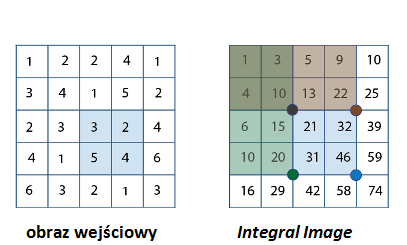
\includegraphics[width=12cm]{integral_image}
	\centering
	\caption{Zasada wyliczania obrazu całkowego}
	\label{im: Integral Image}
\end{figure}    

Wyliczenie sumy wyróżnionego regionu na obrazie wejściowym można zastąpić operacjami na obrazie całkowym. Sumę obszaru można uzyskać korzystając z czterech wartości powyżej oraz na lewo od zaznaczonych kropek: \textit{46 - 22 - 20 + 10 = 14}. Jak nietrudno obliczyć, wynik ten jest równy sumie zaznaczonych elementów obrazu wejściowego.

\section{Ciągła przestrzeń skali dla obrazu}
\label{sec:StateSpace}
W cyfrowym przetwarzaniu obrazów model ciągłej przestrzeni skali może zostać użyty do reprezentacji obrazu jako rodziny stopniowo rozmywających się obrazów. Wykorzystanie ciągłej przestrzeni skali umożliwia znalezienie punktów na obrazie, które są niewrażliwe na zmiany skali (z ang. \textit{scale invariant}). 

To zagadnienie jest bardzo ogólne i istnieje wiele reprezentacji przestrzeni skali. Typowym podejściem do zdefiniowania szczególnej reprezentacji przestrzeni skali jest zdefiniowanie zbioru aksjomatów opisujących podstawowe własności szukanej przestrzeni. Najbardziej powszechnym zbiorem aksjomatów jest zbiór definiujący liniową przestrzeń skali powiązaną z funkcją Gaussa. 

\begin{figure}[h]
	%\centering
	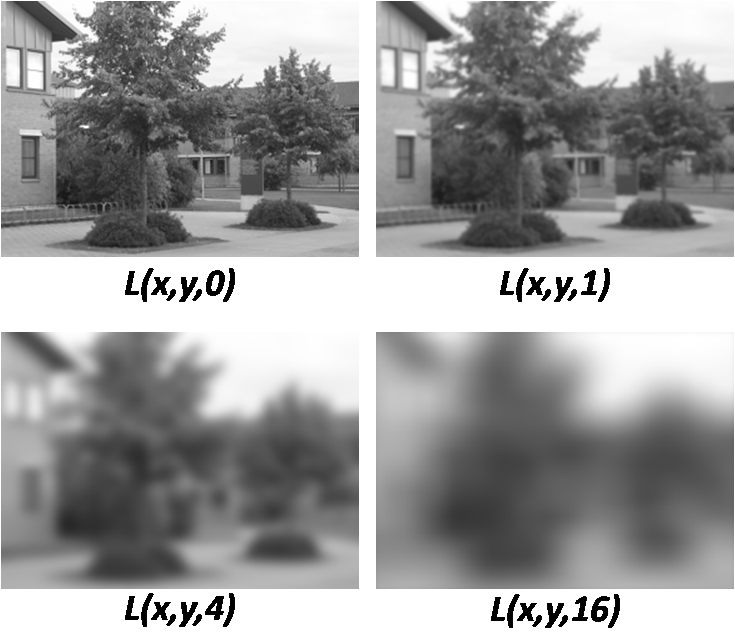
\includegraphics[width=10cm]{ScaleSpaceRepresentation}
	\centering
	\caption{Reprezentacja przestrzeni skali dla różnych wartości $\sigma$}
	\label{im: Scale Space Representation}
\end{figure} 

Problem sprowadza się do znalezienia takiego zbioru operatorów $\tau_s$, który operaując na obrazie oryginalnym zdefiniuje zbiór obrazów rozmytych:  

Gaussowska przestrzeń skali (dla obrazu dwuwymiarowego) zdefiniowana jest jako splot obrazu \textit{I(x,y)} z dwuwymiarową funkcją Gaussa \textit{g(x,y,$\sigma$)}:
\begin{equation}
L(x,y,\sigma) = g(x,y,\sigma)*I(x,y)
\end{equation}
gdzie:
\begin{equation}
g(x,y,\sigma) = \frac{1}{2\pi\sigma}e^{-(x^2+y^2)/2\sigma}
\end{equation}

%Podany wzór spełniony jest dla \textit{$\sigma$$\geq$0}
Dla $\sigma = 0$ filtr Gaussa staje się funkcją impulsową, zatem \textit{L(x,y,0) = f(x,y)}. Wraz ze zwiększaniem parametru $\sigma$ przestrzeń skali \textit{L} staje się coraz bardziej rozmyta, czyli coraz mniej szczegółów przestaje być widoczne. Na rysunku \ref{im: Scale Space Representation} przedstawiono przykład tworzenia przestrzennej reprezentacji skali.

\section{Windows Presentation Foundation (WPF)}
\label{sec: WPF}
Windows Presentation Foundation jest silnikiem graficznym dostarczanym przez firmę Microsoft. Jego premiera nastąpiła w 2006 roku, gdy stał się częścią platformy programistycznej .NET w wersji 3.0.  Jest wykorzystywany głównie do budowania aplikacji okienkowych nowej generacji dla systemu opracyjnego Windows. WPF zbudowany został całkowicie niezależnie do dotychczasowego silnika renderujacego GDI. Dostarcza model programistyczny umożliwiajacy budowanie aplikacji oraz pozwalający na bezwzględną separację logiki biznesowej od interfejsu użytkownika. 

\begin{figure}[h]
	%\centering
	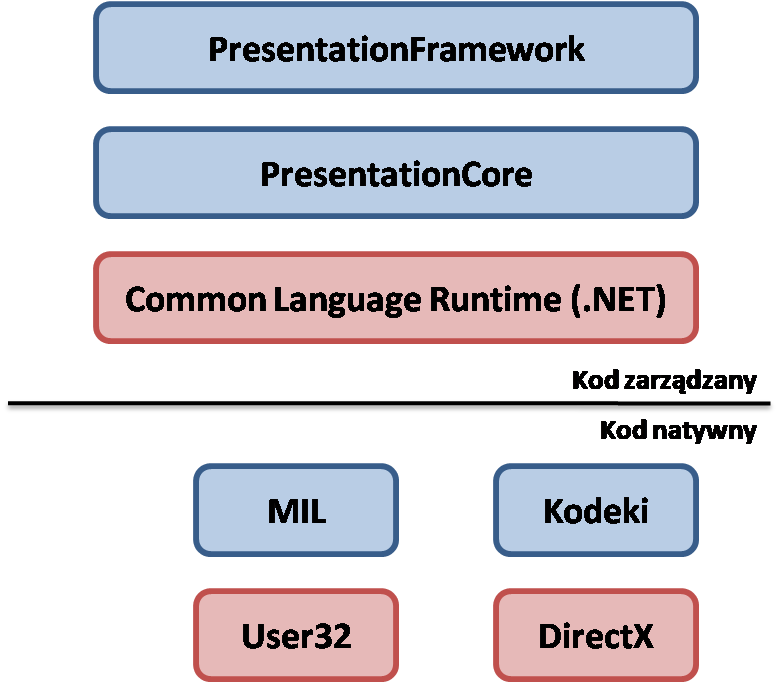
\includegraphics[width=10cm]{WpfArchitecture}
	\centering
	\caption{Architektura WPF. Czerwone elementy to komponenty bibliotek Windows. SKładowe WPF oznaczono kolorem niebieskim.}
	\label{im: WpfArchitecture}
\end{figure} 

Architektura silnika WPF została oparta zarówno o kod zarządzany, jak i o kod natywny.  Większość elementów składowych znajduje się w kodzie zarządzanym, tak jak publiczne API dostępne dla deweloperów. Na rysunku \ref{im: WpfArchitecture} przedstawiono architekturę silnika, w skład którego wchodzą:

\begin{itemize}
	\item PresentationFramework – biblioteka implementująca elementy do prezentacji dla końcowego uzytkownika tj. rozkład kontrolek, wyświetlanie animacji, skalowanie aplikacji. 
	
	\item PresentationCore – podstawowa biblioteka w technologii WPF. Dostarcza wraper dla MIL z poziomu kodu zarządzanego oraz impementuje bazowe  usługi dla każdej aplikacji WPF. W skład tych usług wchodzi przede wszystkim system zarządzania wiadomościami , którego implementację stanowi obiekt typu Dispacher.  
	
	\item Media Integration Layer, MIL – komponent działający w kodzie niezarządzanym w celu zapewnienia wydajnej współpracy  z DirectX.   Zawiera silnik kompozycji, który odpowiada za  podstawową obsługę renderowania powierzchni 2D oraz 3D.
	
	\item Kodeki – zbiór programów odpowiedzialnych do przekształcania strumienia danych do postaci multimedialnej.
	
	\item DirectX – kolekcja zawierająca interfejsy programistyczne aplikacji (z ang. application programming interfaces, APIs). Zestaw ten  wspomaga generację grafiki, dźwięku oraz innych elementów związanych z aplikacjami multimedialnymi
	
	\item User32 – komponent Microsoft Windows dostarczający bazowe funkcjonalności do tworzenia prostych interfejsów użytkownika.  Aplikacje WPF zawierają obiekt typu Dispacher, który używa systemu zarządzania wiadomościami dostępnymi w User32.
	
	\item Common Language Runtime, CLR – wspólne środowisko uruchomieniowe. Podstawowy komponent .NET. Pelni wiele kluczowych roli tj. uruchomienie aplikacji, zarządzanie pamięcią. Dodatkowo zajmuje się również konwersja języka IL do kodu maszynowego. Elementem bazowym środowiska CLR jest standardowy zestaw typów danych, który jest wykorzystywany przez wszyskie języki programowania oparte o CLR. 
	
\end{itemize}

Silnik WPF udostępnia system własności dla obiektów, które dziedziczą z DependencyObject. Obiekt ten monitoruje  wszytkie zależności pomiędzy własnościami i jest w stanie wykonywać odpowiednie akcje bazujac na ich zmianach. Własności implementują mechanizm informujący o zmianach (z ang. Change notifications), który wywołuje wbudowane zachowania (z ang. Behaviors) w przypadku wykrycia jakiejkolwiek zmiany. Dodatkowo isniej możliwość definiowania własnych zachowań w celu propagowania informacji o zmianie własności do innych elementów . System zarządzania rozkładem elementów w obrzarze interfejsu użytkownika wykorzystuje powyższy zbior zachowań do przeliczania nowego rozkładu w przypadku zmiany własności. Dzięki temu architektura systemu WPF spełnia deklaratywny paradygmat programowania, w którym praktycznie wszystko, począwszy od ustawania wielkości kontrolek do tworzenia animacji może zostać osiągnięte poprzez zmianę własności. Takie zachowanie umożliwia tworzenie aplikacji WPF w XAML (z ang. Extensible Application Markup Language) – deklaratywnym języku znaczników, gdzie przy pomocy atrybutów oraz słów kluczowych tworzone jest bezpośrednie połączenie z własnościami oraz klasami technologii WPF. 

Każdy element interfejsu aplikacji WPF dziedziczy z abstrakcyjnej klasy Visual. Obiekty tej klasy dostarczają interfejs do drzewa kompozycji zarządzanego przez MIL. Każdy element WPF tworzy oraz dodaje przynajmniej jeden węzeł kompozycji do drzewa. Węzły te zawierają przede wszystkim instrukcje renderowania takie jak przycinanie elementu bądź transformacja wizualna. Zatem cała aplikacja może być traktowana jako kolekcja węzłów kompozycji, które są przechowywane w buforze pamięci. Okresowo MIL przechodzi po strukturze drzewa i wykonuje instrukcje renderowania dla każdego węzła. Powoduje to tworzenie kompozytu na powierzchni DirectX, która następnie jest wyświetlana na ekranie.  MIL wykorzystuje algorytm malarza, w którym wyświetlanie elementów na monitorze rozpoczyna się od tych najbardziej odległych (tło). Takie zachowanie umożliwia renderowanie złożonych efektów takich jak rozmycie czy transparentność. Dodatkowo proces rysowania jest sprzętowo wspomagany przy pomocy GPU. 

Każda z aplikacji WPF staruje z dwoma wątkami: pierwszy służy do obsługi interfejsu użytkownika, a drugi, działający w tle, obsługuje renderowanie oraz przerysowywanie – jego działanie jest automatyczne, więc nie wymaga żadnej interwencji dewelopera. Wątek powiązany z UI przechowuje obiekt Dispacher’a (poprzez instancję klasy DispacherObject), który zajmuje się kolejkowaniem operacji koniecznych do wykonania na interfejsie użytkownika.

Etap tworzenia układu interfejsu użytkownika podzielony jest na dwie fazy: Mierzenie (z ang. Measure) oraz Porządkowanie (z ang. Arrange). Faza mierzenia rekursywnie wywołuje wszystkie elementy określa rozmiar, z jakim one będą wyświetlane. Porządkowanie to faza, podczas której następuje rekursywne układanie wszystkich elementów w stosunku do ich rodziców w drzewie kompozycji. 


\section{Algorytm SURF}
Algorytm SURF (skrót od ang. \textit{Speeded Up Robust Features}) został opatentowany przez grupę naukowców w 2007 roku [BIBLIOGRAFIA]. Należy do rodziny algorytmów bazujących na punktach kluczowych i służy do porównywania dwóch obrazów operując w odcieniach szarości. W celu znalezienia cech obrazu niezależnych od zmiany skali wykorzystuje opisaną w podrozdziale \ref{sec:StateSpace} technikę utworzenia ciągłej przestrzeni skali opartej na rozkładzie Gaussa. 
%Dodatkowo algorytm ten dzieli przestzeń skali na poziomy oraz oktawy. Oktawa odpowiada zbiorowi splotów, w którym wartość parametru $\sigma$ zostaje podwojona. Każda oktawa podzielona jest na jednakowo odległe (ze względu na parametr $\sigma$) poziomy. Przykład przedstawiono na rysunku \ref{im: OctavesAndLevels}.

Działanie algorytmu można podzielić na 3 etapy:
\begin{itemize}
	\item Detekcja (z ang. \textit{Detection}) – faza automatycznej identyfikcji punktów kluczowych (z ang. \textit{interest points}). Te same punkty powinny zostać wykryte niezależnie od zmian w położeniu, naświetleniu oraz orientacji obrazu, również w pewnym stopniu od zmiany skali oraz punktu widzenia. 
	\item Opis (z ang. \textit{Description}) – każdy punkt kluczowy powinien zostać opisany w unikatowy sposób., aby był niezależny od rotacji oraz przeskalowaniu obrazu.
	\item Zestawienie (z ang. \textit{Matching}) – faza, podczas której określa się (na podstawie podanych punktów kluczowych) jakie obiekty znajdują się na obrazie. 
\end{itemize}

W dalszej części rozdziału przedstawiono bardziej dokładną analizę dwóch pierwszych etapów.

\subsection{Detekcja}
Algorytm SURF do wykrycia punktów kluczowych wykorzystuje wyznacznik Hesjanu. Dokładniej rzecz ujmując, metoda ta wyszukuje na obrazie regionów, w których wyznacznik macierzy Hessego jest maksymalny. 






%Najważniejszy element detekcji to proces polegający na ograniczaniu lokalnych wartości niemaksymalnych (z ang. \textit{non-maximal suppression}) dla wyznaczników macierzy Hessego przy różnych wartościach parametru $\sigma$. W celu redukcji czasu obliczeń korzysta z obrazu całkowego opisanego w podrozdziale \ref{sec:IntegralImage}.

Mając do dyspozycji punkt \textit{\textbf{x}=(x,y)} z obrazu całkowego, macierz Hessego \textit{H(\textbf{x},$\sigma$)} dla skali $\sigma$ jest zdefiniowana następująco:
\begin{equation}\textsl{}
H(\textbf{x},\sigma) = 
\begin{bmatrix}
L_{xx}(\textbf{x},\sigma) & L_{xy}(\textbf{x},\sigma) \\ L_{xy}(\textbf{x},\sigma) & L_{yy}(\textbf{x},\sigma)
\end{bmatrix}
\end{equation}

gdzie 
\begin{equation}\textsl{}
L_{xx}(\textbf{x},\sigma) = I(\textbf{x})*\frac{\delta^2}{\delta x^2}g(\sigma)
\end{equation}
\begin{equation}\textsl{}
L_{xy}(\textbf{x},\sigma) = I(\textbf{x})*\frac{\delta^2}{\delta xy}g(\sigma)
\end{equation}

Udowodniono, że przestrzeń skali oparta o funkcję Gaussa jest rozwiązaniem optymalnym {BIBLIOGRAFIA}, jednakże w zastosowaniach praktycznych wyliczanie splotu jest niezwykle kosztowne obliczeniowo. W celu przyspieszenia obliczeń dokonano aproksymacji drugich pochodnych cząstkowych filtrami przedstawionymi na rysunku \ref{im: GaussianApproximation}. Dodatkowo wykorzystanie obrazu całkowego powoduje, że czas wyliczania splotów nie zależy od wielkości filtra. 
\begin{figure}[h]
	%\centering
	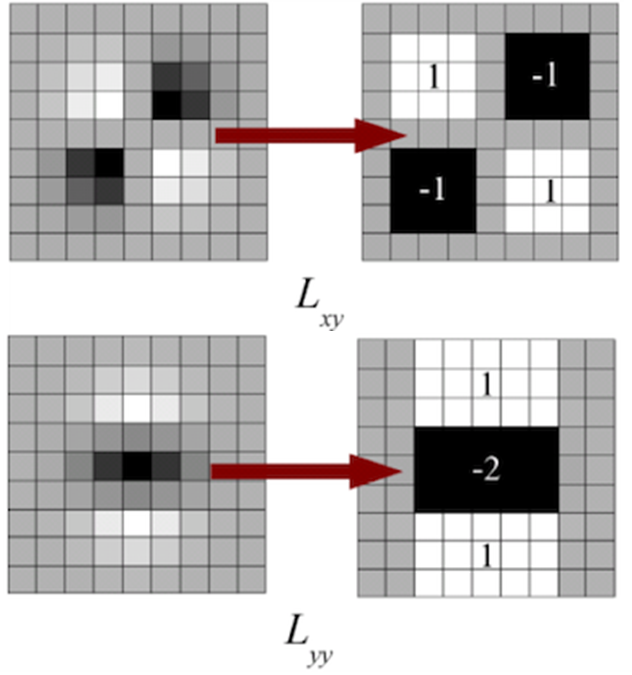
\includegraphics[width=8cm]{SurfLxyLyy}
	\centering
	\caption{Dwa rysunki po lewej to sploty \textit{$L_{xy}$} oraz \textit{$L_{yy}$} poddane dyskretyzacji oraz przycięciu. Po prawej stronie przedstawiono aproksymacje wyżej wymienionych splotów (odpowiednio \textit{$D_{xy}$} oraz \textit{$D_{yy}$}). Szare regiony są równe zero [BIBLIOGRAFIA]}
	\label{im: GaussianApproximation}
\end{figure}

Przedstawione filtry o rozmiarze \textit{9 x 9} odpowiadają splotom, dla których parametr $\sigma$ jest równy 1.2. Jest to najmniejsza wartość skali, dla której algorytm SURF może dawać zadowalające rezultaty.

Biorąc pod uwagę powyższe założenia, wyznacznik aproksymowanej macierzy Hessego wynosi:
\begin{equation}\textsl{}
det(H_{aproks}) = D_{xx}D_{yy} - (wD_{xy})^2.
\end{equation}
Aby uczynić aproksymację Hesjanu bardziej dokładną wprowadzono parametr \textit{w}. Teoretycznie jest on zależny od skali, jednakże badania wykazały [BIBLIOGRAFIA], że można uczynić go stałą równą \textit{0.9}.  
Wynikiem powyższych działań jest uzyskanie aproksymowanego wyznacznika Hesjanu dla każdego punktu obrazu \textit{\textbf{x}} przy różnych wartościach parametru $\sigma$.

 Algorytm SURF dzieli przestrzeń skali na oktawy. Oktawa reprezentuje zbiór odpowiedzi filtrów otrzymanych przez splot obrazu z filtrami coraz większych rozmiarów. Każda oktawa odpowiada fragmentowi przestrzeni skali, w którym nastąpiło podojenie parametru $\sigma$ oraz jest podzielona na stałą liczbę poziomów. Wraz ze wzrostem wielkości filtrów musi zostać spełnione dwa założenia: o istnieniu piksela centralnego oraz o zachowaniu proporcji poszczególnych obszarów maski. W pracy [BIBLIOGRAFIA] opisano szczegółowo, w jaki sposób definiować oktawy oraz liczbę poziomów dla nich. Przykład poprawnego skalowania filtra przedstawiono na rysunku \ref{im: FiltersScale}. 
 
 \begin{figure}[h]
 	%\centering
 	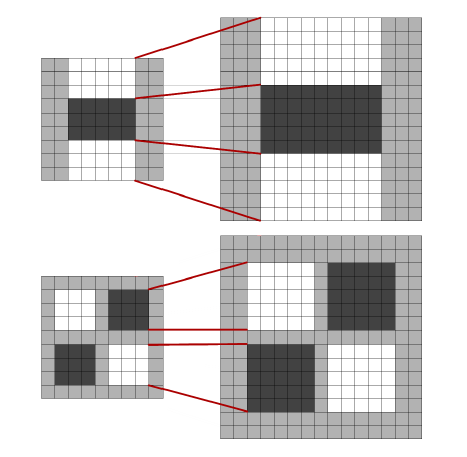
\includegraphics[width=12cm]{FiltersScale}
 	\centering
 	\caption{Filtr $D_{yy}$ oraz $D_{xy}$ dla dwóch kolejnych poziomów w oktawie (\textit{9 x 9} oraz \textit{15 x 15}). Długość czarnego regionu dla górnego filtra może zostać zwiększona tylko o parzystą liczbę pikseli w celu zagwarantowania istnienia piksela centralnego.}
 	\label{im: FiltersScale}
 \end{figure}
 
W celu zlokalizowania punktów kluczowych na obrazie we wszystkich skalach, algorytm SURF wykorzystuje ograniczanie lokalnych wartości niemaksymalnych (z ang. \textit{non-maximal suppression}) dla obszaru wielkości \textit{3 x 3 x 3} piksele. Zasada działania została opisana w pracy [BIBLIOGRAFIA]. Następnie maksima wyznacznika Hessjanu dla poszczególnych skal sa interpolowane na obraz oryginalny.

\subsection{Deskryptor} 
Aby punkt kluczowy był niewrażliwy na zmiany orientacji, punktowi przypisywana zostaje orientacja. W tym celu algorytm SURF wylicza odpowiedź falki Haara dla kolistego otoczenia punktu orientacji. Falka jest wyliczana w kierunku poziomym (\textit{dx}) oraz pionowym (\textit{dy}) dla każdego elementu z otoczenia punktu kluczowego.
Główna orientacja jest wyliczana następująco: mając odpowiedzi falki Haara dla każdego punktu z otoczenia, skonstruowano przesuwne okno o kącie rozwarcia równym 60 stopni. Dla każdego okna wyliczano sumę wszystkich elementów, a maska zostaje przesunięta. Najdłuższy znaleziony wektor stanowi główną orientację znalezionego punktu kluczowego. Szczegóły na rysunku \ref{im: SurfOrientationTwo}.

 \begin{figure}[h]
	%\centering
	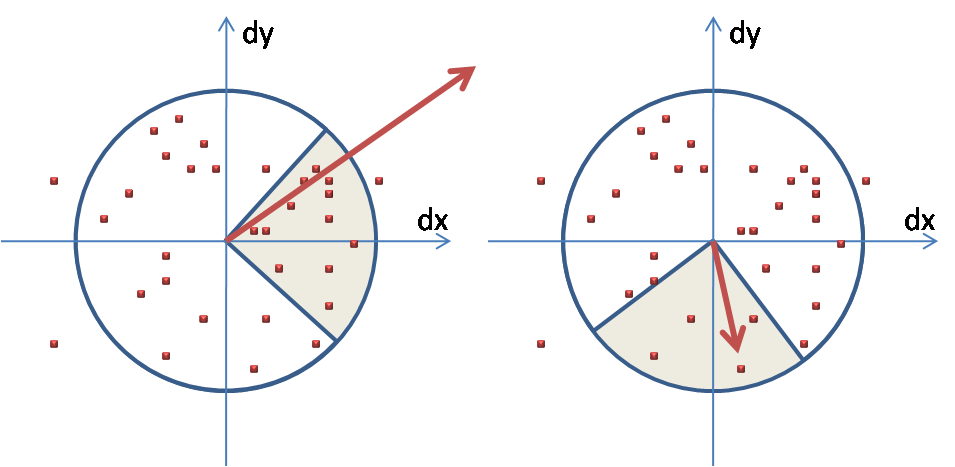
\includegraphics[width=12cm]{SurfOrientationTwo}
	\centering
	\caption{Przypisanie orientacji. Okno o kącie rozwarcia 60 stopni obraca się wokół początku układu współrzędnych, a wyliczone odpowiedzi falki Haara zostają sumowane tworząc wektory oznaczone kolorem czerwonym. Najdłuższy wektor determinuje główną orientację punku kluczowego.}
	\label{im: SurfOrientationTwo}
\end{figure}

Kolejnym etapem tworzenia deskryptora jest podzielenie obszaru wokół punktu kluczowego na  \textit{4 x 4} kwadratowe obszary. Taki podział zachowuje istotne przestrzenne informacje. Każdy z podregionów zawiera \textit{5 x 5} punktów rozmieszczonych regularnie w wierzchołkach siatki. Dla każdego punktu wyliczone zostają odpowiedzi falki Haara w kierunku poziomym oraz pionowym. Odpowiedzi te uwzględniają rotację całego obszaru zgodnie z orientacją badanego punktu kluczowego. Schemat przedstawiono na rysunku \ref{im: Description}. Następnie odpowiedzi \textit{dx} oraz \textit{dy} są sumowane dla każdego z podregionów. Stanowią one pierwszą część deskryptora cechy. Dodatkowo w celu uwzględnienia informacji o zmianach intensywności wyliczane są sumy modułów odpowiedzi falki Haara. 

Zatem, dla każdego z podregionów otrzymano czterowymiarowy wektor opisujacy o strukturze \textit{\textbf{v} = ($\sum$$d_x$, $\sum$$d_y$, $\sum$$|d_x|$, $\sum$$|d_y|)$}. Uwzględniając wszystkie podregiony, punkt kluczowy opisany jest 64-elementowym wektorem. 

 \begin{figure}[h]
	%\centering
	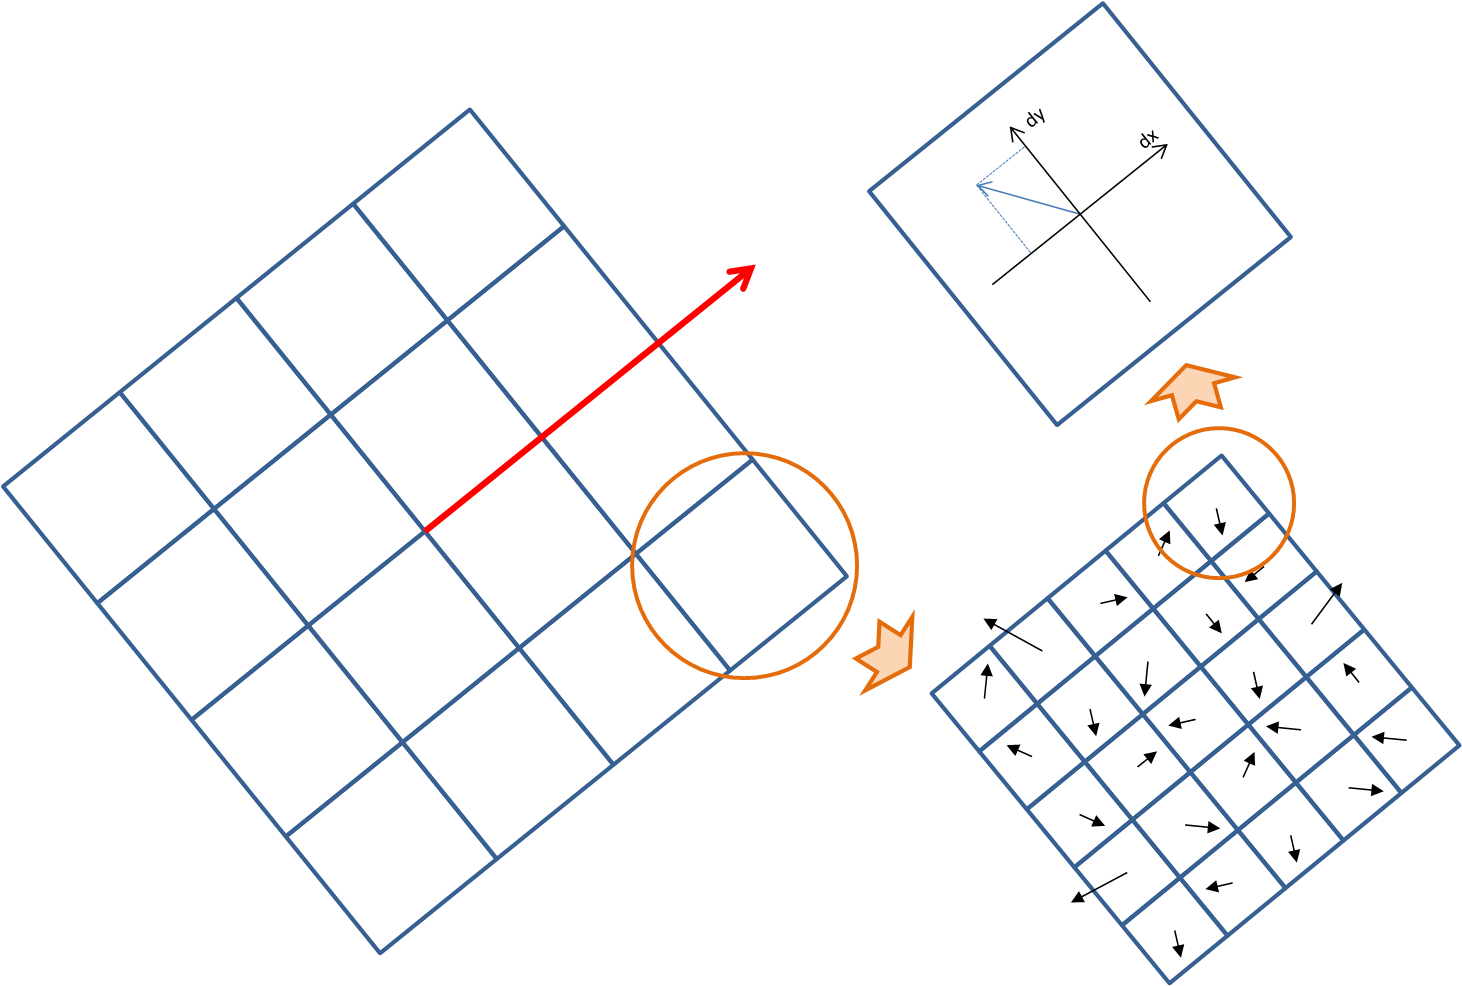
\includegraphics[width=16cm]{Description}
	\centering
	\caption{Tworzenie deskryptora. Otoczenie punktu kluczowego obrócono zgodnie z orientacją cechy. Dla wszystkich elementów podregionu wyliczono odpowiedź falki Haara w dwóch kierunkach.}
	\label{im: Description}
\end{figure}

MOŻNA DOPISAC O ZNAKU LAPLASJANU I O ROZRZERZENIU DO 128 ELEMENTOW.

\section{Accord .NET}
Accord .NET jest to szkielet aplikacyjny oparty o środowisko .NET. Zawiera biblioteki implementujące bardzo wiele algorytmów z szerokiej listy dziedzin nauki takich jak:

\begin{itemize}
	\item klasyfikacja: sieci neuronowe, metody wektorów nośnych (z ang. Support Vector Machine, SVM), algorytm Levenberga-Marquardta, model Markova, tworzenie drzew decyzyjnych
	\item regresja: regularyzacja, regresja liniowa, wielomianowa, 
	\item analiza skupień (z ang. \textit{clustering}): algorytm k-średnich, podział binarny. 
	\item rozkład prawdopodobieństwa: rozkład normalny, Poissona, Cauchy'ego
	\item Przetwarzanie obrazów cyfrowych (z ang. \textit{digital image processing, DIP}): deskryptory punktów kluczowych - SURF, FREAK, FAST; deskryptory gęstości - HOG, LBP
	\item Rozpoznawanie obrazów (z ang. computer vision): metody do detekcji, śledzenia oraz transformacji obiektów w strumieniu wideo. 
\end{itemize}

Szkielet ten został zaimplementowany aby rozszerzyć możliwości istniejącego rozwiązania - AForge .NET, jednak z czasem oba podmioty zostały ze sobą połączone pod jedną nazwą Accord .NET. Framework jest dostępny do pobrania z poziomu kodu zródłowego jak również za pomocą systemu zarządzania pakietami - \textit{NuGet}.

\section{C\#}
 C\# jest językiem programowania spełniającym wiele paradygmatów takich jak programowanie funkcyjne, obiektowe, imperatywne czy generyczne. Został utworzony przez firmę \textit{Microsoft} wewnątrz platformy .NET i zatwierdzony jako standard przez ISO (ISO/IEC 23270:2006) oraz Ecma (ECMA-334). Jest jednym z języków wchodzącym w skład Architektury Wspólnego Języka (z ang. \textit{Common Language Infrastructure, }). Najnowsza wersja języka to C\# 7.3, która ukazała się w 2018 roku wraz z środowiskiem programistycznym \textit{Visual Studio 2017} w wersji 15.7.2.
 Przykładowe cechy języka C\#:
 \begin{itemize}
 	\item C\# z założenia ma być językiem prostym, nowoczesnym, obiektowym
 	\item Język posiada hierarchię klas, a wszystkie elementy (nawet najprostsze typy) dziedziczą z klasy \textit{System.Object}.
 	\item Język ma zapewniać wsparcie w tworzeniu oprogramowania, w skład którego wchodzą: sprawdzanie silnego typowania, kontrola zakresu tablic, detekcja prób użycia niezainicjowanych zmiennych.
 	\item Automatyczne odśmiecanie pamięci (usuwanie nieużywanych elementów) - wykorzystanie mechanizmu \textit{Garbage Collector}.
 	\item Wielodziedziczenie, czyli dziedziczenie od więcej niż jednej klasy jest niedozwolone. Wielokrotne dziedziczenie jest możliwe jedynie po interfejsach.
 	\item Wsparcie dla internacjonalizacji.
 	\item Przenośność oprogramowania oraz łatwość wdrożenia w rozproszonych środowiskach. 
 	\item Język C\# jest bezpieczny w kontekście konwersji typów. Automatyczna konwersja jest dokonywana tylko w przypadku, gdy dane rzutowanie jest uznawane za bezpieczne.
 	\item Mechanizm refleksji oraz dynamicznego tworzenia kodu. Takie wsparcie umożliwia tworzenie oprogramowania, którego części nie jest w całości znane podczas kompilacji.
 	Takie działanie jest szeroko wykorzystywane w procesie mapowania obiektowo-relacyjnego (z ang. Object-Relational Mapping, ORM).
 \end{itemize} 

\section{.NET}
Platforma programistyczna .NET została zaprojektowana przez firmę \textit{Microsoft}. Zawiera w sobie obszerną bibliotekę klas FCL (z ang. \textit{Framework Class Library}) oraz zapewnia kompatybilność dla kilku języków programowania. Programy napisane z wykorzystaniem .NET są wykonywane w środowisku CLR (z ang. \textit{Common Language Runtime}) - jest to maszyna wirtualna, która dostarcza usługi takie jak bezpieczeństwo, zarządzanie pamięcią czy obsługę wyjątków. 
W skład architektury wchodzą: MOŻNA COS DOPISAĆ


Cechy platformy .NET:
\begin{itemize}
	\item Głównym elementem platformy .NET jest Środowisko Uruchomieniowe Wspólnego Języka (z ang. \textit{Common Language Runtime}, CLR). Stanowi ono implementację CLI gwarantując wiele właściwości oraz zachowań w obszarach zarządzania pamięcią bądź bezpieczeństwa. Głównym zadaniem komponentu CLR jest zamiana skompilowanego kodu CIL (z ang. Common Intermediate Language) na kod maszynowy, który jest dostosowany do maszyny, na jakiej został uruchomiony. MOŻE RYSUNEK?
	\item Kompatybilność wsteczna: ponieważ systemu komputerowe bardzo często wymagają interakcji pomiędzy nowszymi i starszymi komponentami, platforma .NET daje możliwość wykonywania funkcji poza platformą. Dostęp do komponentów COM jest możliwy dzięki wykorzystaniu przestrzeni nazw \textit{System.Runtime.InteropServices} oraz \textit{System.EnterpriseServices}.
	\item W skład platformy .NET wchodzi komponent CTS (z ang. \textit{Common Type System}), który definiuje wszystkie możliwe typy danych wspierane przez CLR oraz w jaki sposób mogą one ze sobą ingerować. Dzięki temu jest możliwa wymiana typów bądz instancji obiektów pomiędzy bibliotekami oraz aplikacjami napisanymi w różnych językach opartych o .NET.
	\item Przenośność: platforma została zaprojektowana w taki sposób, aby jej implementacja była możliwa dla różnych systemów operacyjnych.
	\item Bezpieczeństwo: platforma .NET dostarcza wspólny model bezpieczeństwa dla programów tworzonych w jej ramach. Została zaprojektowana w taki sposób, aby uniknąć wielu problemów z bezpieczeństwem aplikacji, do których należy m.in. przepełnienie bufora, które jest bardzo często używane przez złośliwe oprogramowanie (z ang. \textit{malicious software}, w skrócie \textit{malware}).
	
\end{itemize}

\section{Microsoft Visual Studio}
Microsoft Visual Studio to zintegrowane środowisko programistyczne (z ang. \textit{Integrated Deveopment Environment, IDE}) dostarczane prze firmę \textit{Microsoft}. Służy do budowania aplikacji konsolowych, jak również stron internetowych, aplikacji webowych oraz mobilnych. Visual Studio używa dostarczanych przez firmę Microsoft platform do tworzenia oprogramowania, do których należą m.in Windows Forms oraz Windows Presentation Foundation. Umożliwia tworzenie oprogramowania w 36 różnych językach programowania tj: C\#, C, C++, Visual Basic .NET, JavaScript czy CSS. Obecnie najnowsza wersja to Visual Studio 2017. 

Jednym z najważniejszych elementów wchodzących w skład środowiska jest edytor kodu. Jak każde IDE, Visual Studio zawiera edytor umożliwiający podświetlanie składni oraz auto-uzupełnianie brakujących fraz wykorzystując mechanizm \textit{IntelliSense}. Środowisko programistyczne wspiera tzw. kompilację w tle. W trakcie pisania kodu, Visual Studio kompiluje kod w tle w celu dostarczenia informacji o składni oraz ewentualnych błędach kompilacji. 

Visual Studio zawiera debugger umożliwiający redukcję błędów w oprogramowaniu zarówno dla kodu zarządzanego, jak i natywnego. Dodatkowo istnieje możliwość dopięcia debuggera do procesu w celu monitorowania zachowania. Visual Studio umożliwia dokonywania zrzutów pamięci (z ang. \textit{memory dumps}) jak również wczytywania ich w dalszych momentach debugowania. Debugger umożliwia tworzenie punktu wstrzymania (z ang. \textit{breakpiont}) - miejsca celowego zatrzymania wykonywania programu w celu analizy jego zachowania. Dodatkowo punkty wstrzymania mogą być warunkowe, czyli zatrzymanie w punkcie następuje w momencie spełnienia warunku. Debugger wspiera tzw. "Edytuj i Kontynuuj" - jak nazwa sugeruje, istnieje możliwość zmiany wartosci zmiennej podczas procesu debugowania.

Visual Studio zawiera narzędzia do tworzenia interfejsu użytkownika. Jeden z przykładów może stanowić narzędzie \textit{Cider} pomocne w budowaniu aplikacji WPF. Umożliwia tworzenie aplikacji poprzez przeciąganie istniejących elementów z przybornika oraz ustawianiu ich własciwości w dedykowanym oknie. Ponadto istnieje możliwość edycji widoku z poziomu języka znaczników XAML. Szczegółowy opis technologii WPF znajduje się w podrozdziale \ref{sec: WPF}.\textsl{}

\section{Algorytm centroidów}
Algorytm K-średnich (z ang. \textit{K-means}) jest jedną z najprostszych metod klasyfikacji bez nadzoru (z ang. \textit{unsupervised learning}). Grupowanie elementów oparte jest o wstępne podzielenie zbioru danych na z góry założoną liczbę klastrów. W kolejnych krokach niektóre z elementów skupień są przenoszone do innych klastrów w taki sposób, aby wariancja wewnątrz każdej z grup była jak najmniejsza. Minimalizacja wartosci wariancji powoduje, że elementy wewnątrz poszczególnych klastrów są do siebie maksymalnie podobne. 

\begin{enumerate}
	\item Wybór centroidów klastrów: dla podanej z góry liczby klas (skupień)  środki klastrów powinny zostać dobrane w taki sposób, aby były możliwie jak najdalej od siebie.
	\item Przyporządkowanie każdego elementu ze zbioru danych do najbliższego środka klastra, normę może stanowić odległość euklidesowa lub Czebyszewa.
	\item Ponowne wyliczenie środków skupień: w większości zastosowań nowym środkiem klastra jest punkt o współrzędnych stanowiących średnią arytmetyczną elementów wewnątrz skupienia.
	\item Powtarzanie algorytmu do momentu osiągnięcia kryterium zbieżności: sytuacja, podczas której środki klastrów pozostają bez zmian bądź nie zmienia się przynależność elementów do klas.
\end{enumerate}

Na rysunku \ref{im: Clustering} przedstawiono graf przepływu wyjaśniający zasadę działania algorytmu K-średnich.
\begin{figure}[h]
	%\centering
	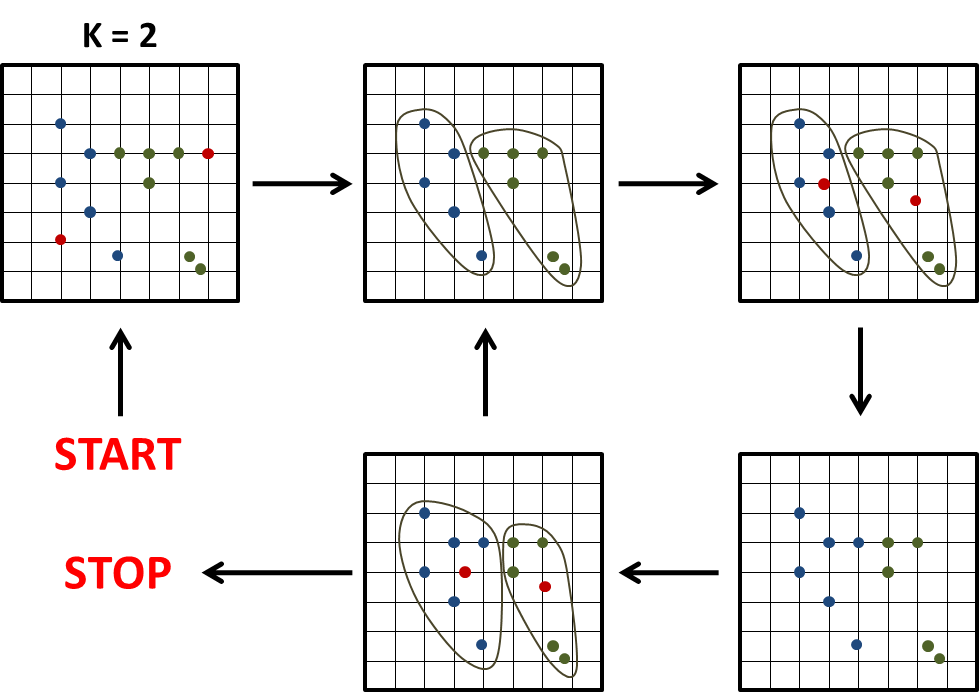
\includegraphics[width=16cm]{Clustering1}
	\centering
	\caption{Algorytm K-średnich. Pierwszy etap to wybór środków dla klastrów. Następnie dokonywane jest przypisanie punktów do odpowiedniej klasy. Kolejny etap to ponowne wyliczenie centroidów oraz reorganizacja klastrów. Algorytm działa dopóki środki klas ulegają zmianie.}
	\label{im: Clustering}
\end{figure}


\section{Metoda Wektorów Nośnych}
\label{sec: SVM}
Metoda wektorów nośnych (z ang. \textit{Support Vector Machine}, SVM) to jeden z modeli uczenia maszynowego służący do klasyfikacji danych. Model SVM po raz pierwszy został opublikowany przez dwóch naukowców: Vladimira N. Vapnika oraz Alexey'a Chervonenkisa w 1963 roku. Może zostać użyty do rozwiązywania takich problemów jak rozpoznawanie tekstu pisanego czy klasyfikacja obrazów.

Mając do dyspozycji zbiór punktów uczących, w którym każdy z elementów należy do jednej z dwóch klas, SVM tworzy model, który przypisuje próbki testowe do jednej z dwóch kategorii. Model SVM jest reprezentowany jako zbiór punktów na przestrzeni skonstruowany w taki sposób, aby istniała wyraźna przerwa oddzielająca elementy rożnych klas. W zależności od tego, po której stronie przerwy próbka testowa została umiejscowiona, do tej kategorii zostanie przypisana. Bardziej formalnie SVM konstruuje hiperpłaszczyznę rozdzielającą zbiór próbek uczących. Najlepsza separacja zachodzi wtedy, gdy odległość hiperpłaszczyzny od najbliższego elementu dla każdej z klas jest maksymalna. 

Zbiór $n$-punktów uczących opisano następująco:
\begin{equation}
(\vec{x}_1,y_1), ..., (\vec{x}_n,y_n)
\end{equation}
gdzie $\vec{x}_i$ oznacza \textit{\textbf{p}}-wymiarowy wektor. Zmienna $y_i$ przyjmuje wartości -1 bądź 1 w zależności od tego, do której kategorii należy $\vec{x}_i$. Równianie płaszczyzny może zostać opisane następująco:
\begin{equation}
\vec{w}\cdot \vec{x} - b = 0
\end{equation}
gdzie $\vec{w}$ oznacza wektor normalny do szukanej hiperpłaszczyzny. W przypadku, gdy zbiór danych może być separowany liniowo, istnieje możliwość wyboru dwóch równoległych hiperpłaszczyzn, których odległość względem siebie jest maksymalna. Region leżący pomiędzy tymi hiperpłaszczyznami jest nazywany \textit{marginesem}, a optymalna hiperpłaszczyzna leży w jego połowie. Równania dla dwóch równoległych hiperpłaszczyzn są opisane następująco:
\begin{equation}
\vec{w}\cdot \vec{x}_i - b = 1
\end{equation}
\begin{equation}
\vec{w}\cdot \vec{x}_i - b = -1
\end{equation}
Dystans pomiędzy dwoma hiperpłaszczyznami jest równy $2 /||\vec{w}||$. Zatem w celu maksymalizacji dystansu pomiędzy płaszczyznami należy dokonać minimalizacji $||\vec{w}||$. Dodatkowo wymuszono obecność dowolnej próbki po właściwej stronie marginesu używając następujących zależności:
\begin{equation}
\vec{w}\cdot \vec{x}_i - b \geq 1 \hspace{0.5cm} dla \hspace{0.5cm} y_i = 1 
\end{equation}
\begin{equation}
\vec{w}\cdot \vec{x}_i - b \leq -1 \hspace{0.5cm} dla \hspace{0.5cm} y_i = -1
\end{equation}
Powyższe nierówności mogą zostać przekształcone do:
\begin{equation}
y_i(\vec{w}\cdot \vec{x}_i - b) \geq 1 \hspace{0.5cm} dla \hspace{0.2cm} wszystkich \hspace{0.2cm} 1 \leq i \leq n
\end{equation}
Zadanie minimalizacji może zostać postawione w następujący sposób:
"Minimalizacja normy wektora $\vec{w}$ dla zależności $y_i(\vec{w}\cdot \vec{x}_i - b) \geq 1$ dla $i=1 \ldots n$".
Szczegóły tworzenia hiperprzestrzeni w dwóch wymiarach przedstawiono na rysunku \ref{im: SvmMargin}
\begin{figure}[h]
	%\centering
	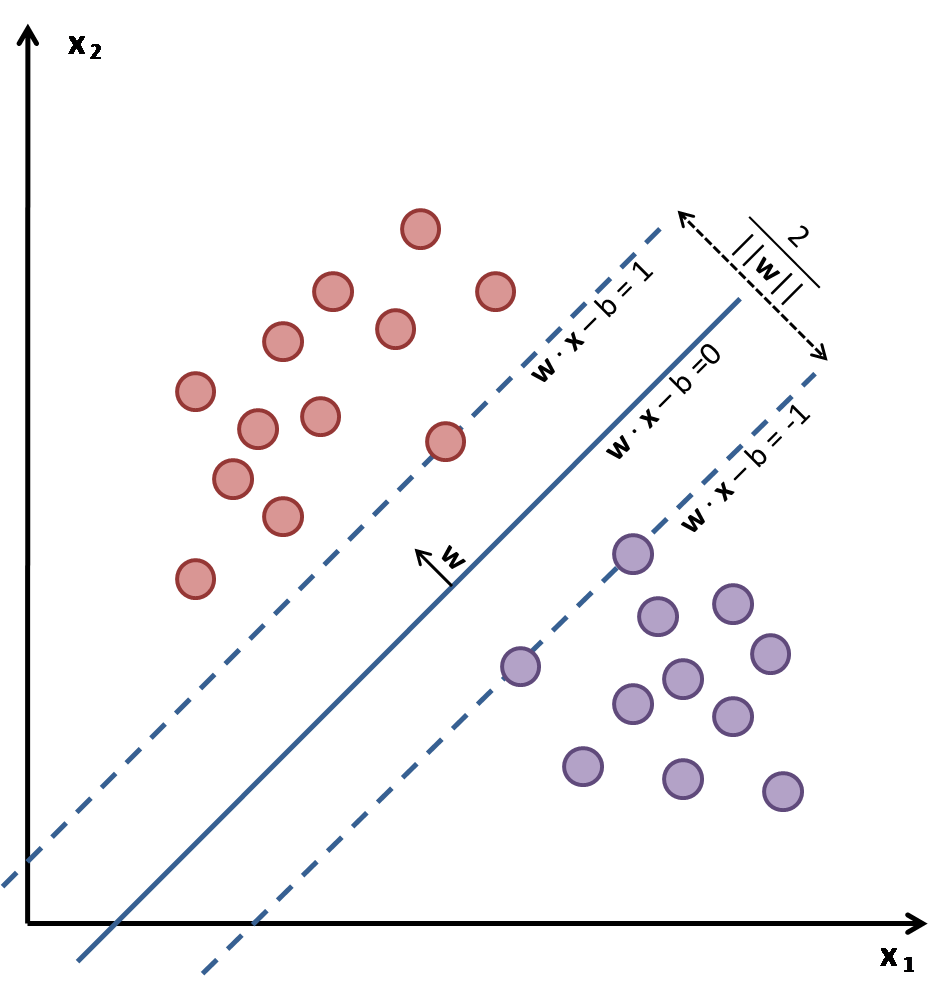
\includegraphics[width=12cm]{SvmMargin}
	\centering
	\caption{Sposób wyznaczania optymalnej hiperpłaszczyzny.}
	\label{im: SvmMargin}
\end{figure}

Oryginalny algorytm do szukania hiperpłaszczyzny rozdzielającej z maksymalnym marginesem stworzony w 1963 roku był liniowym klasyfikatorem. Jednakże w latach 90-tych Vapnik przy wsparciu innych naukowców zaproponował sposób umożliwiający konstrukcję nieliniowego klasyfikatora przez zastosowanie tzw. \textit{"kernel trick"}. Algorytm w swoim działaniu jest bardzo podobny do oryginału z tą różnicą, że każdy iloczyn skalarny zostaje zastąpiony przez nieliniową funkcję jądra. Do najbardziej znanych funkcji jądra należą:

\begin{itemize}
	\item Wielomianowa jednorodna: 
	\begin{equation}
	k(\vec{x}_i,\vec{x}_j) = (\vec{x}_i \cdot \vec{x}_j)^d
	\end{equation}
	\item Wielomianowa niejednorodna:
	\begin{equation}
	k(\vec{x}_i,\vec{x}_j) = (\vec{x}_i \cdot \vec{x}_j + 1)^d
	\end{equation}
	\item Jądro RBF (z ang. Radial Basis Funcion):
	\begin{equation}
	k(\vec{x}_i,\vec{x}_j) = \exp\bigg( -\frac{||\vec{x}_i - \vec{x}_j||^2}{2\sigma^2}\bigg)
	\end{equation}
\end{itemize}
Przykład zastosowania funkcji jądra przedstawiono na rysunku \ref{im: KernelMachine}.
\begin{figure}[h]
	%\centering
	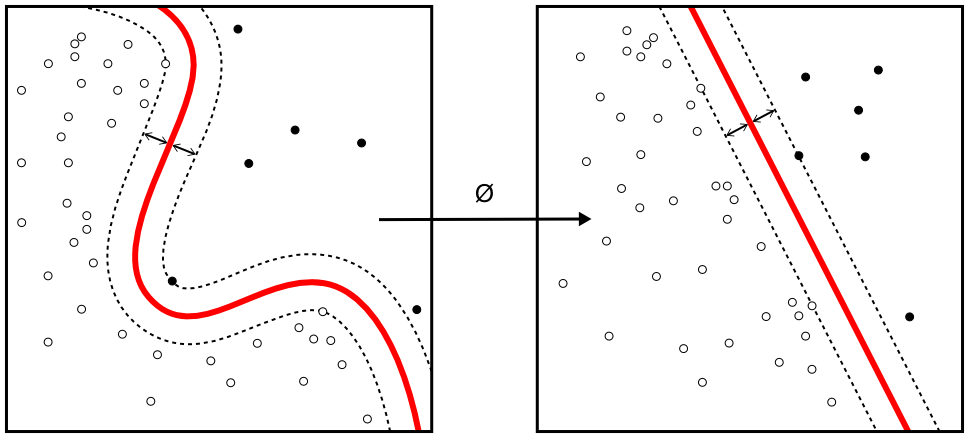
\includegraphics[width=12cm]{KernelMachine}
	\centering
	\caption{Sposób wyznaczania optymalnej hiperpłaszczyzny.}
	\label{im: KernelMachine}
\end{figure}

Istnieje kilka strategii służących do redukcji problemu klasyfikacji dla wielu klas. Do najpopularniejszej metody należy redukcja takiego problemu do wielu przypadków dwuklasowych. Metoda ma dwa warianty: \textit{"jeden-na-resztę"} oraz \textit{"jeden-na-jednego"}. DOPISAĆ

















%\chapter{Technologie i pojęcia wykorzystane w projekcie}


 Protokół Modbus, opisany poniżej, został wykorzystany do wymiany danych między robotem Kawasaki BA006 i aplikacją SCADA. Dodatkowo w poniższym rozdziale przedstawiono sposób kodowania robota oraz wyznaczenie jego położenia.  


\section{Protokół Modbus}

Protokół Modbus został stworzony przez firmę Modicon i opublikowany w 1979 roku. Do dnia dzisiejszego jest on wykorzystywany, szczególnie w aplikacjach przemysłowych do komunikacji pomiędzy urządzeniami elektronicznymi. Standard Modbus definiuje protokół siódmej warstwy modelu OSI in. warstwy aplikacji, który zapewnia komunikację typu klient - serwer pomiędzy urządzeniami mogącymi znajdować się w różnych sieciach. Modbus określa również specjalny protokół dla łącza szeregowego, który umożliwia wymianę żądań wysyłanych pomiędzy urządzeniem typu master, a jednym lub kilkoma urządzeniami typu slave. Specyfikacja ta powoduje, że Modbus klasyfikowany jest również do drugiej warstwy modelu OSI, czyli warstwy łącza danych (rys. \ref{fig:Modbus1}).



\subsection{Komunikacja typu Master-Slave}

Modbus jest protokołem typu Master-Slave. Oznacza to, że w danym czasie do jednej magistrali szeregowej może być podłączony tylko jedno urządzenie typu master oraz klika (maksymalnie 247) urządzeń typu slave. Komunikację zawsze rozpoczyna węzeł typu master. Urządzenia typu slave nigdy nie wysyłają danych bez uprzedniej prośby od węzła typu master, a także nie komunikują się bezpośrednio z innymi urządzeniami typu slave. 

Węzeł typu master może wysyłać żądania do węzłów typu slave w dwóch trybach:

\begin{itemize}
	\item pojedynczej emisji (ang. unicast mode) - master wysyła żądanie do jednego węzła typu slave. Ten z kolei po odebraniu i przetworzeniu żądania wysyła wiadomość zwrotną do mastera. Do tego typu transmisji danych koniecznym jest, aby każde z urządzeń typu slave posiadał swój unikalny adres.
	\item zbiorowej emisji -  (ang. broadcast mode) - master może wysłać żądanie do wszystkich urządzeń typu slave równocześnie. W tym trybie przepływ informacji jest w jedną stronę, to znaczy, że master nie oczekuje na odpowiedzi od węzłów, do których wysłał wiadomość.
\end{itemize}


\subsection{Zasady adresacji}

Przestrzeń adresowa protokołu Modbus składa się z 256 różnych adresów (tab. 3.1). Adres 0 jest zarezerwowany do przesyłu wiadomości w trybie broadcast. Wymagane jest, aby wszystkie urządzenia typu slave rozpoznawały adres 0. Każde z urządzeń slave posiada swój unikalny adres, natomiast master nie ma przypisanego żadnego adresu.


\subsection{Opis pojedynczej ramki}

Dla warstwy aplikacji modelu OSI protokół Modbus definiuje przesyłaną wiadomość in. ramkę, jako pojedynczą jednostkę danych (ang. Protocol Data Unit PDU). Ramka ta jest niezależna od niższych warstw komunikacyjnych i składa się z kodu funkcji (ang. Function code) oraz danych (ang. Data), co przedstawia rysunek \ref{fig:Modbus3}.


Jednakże chcąc użyć protokołu Modbus dla warstwy łącza danych należy zdefiniować dodatkowo pola służące do komunikacji czyli pole adresowe (ang. Address field) oraz pole sumy kontrolnej CRC (ang. Error checking), które przedstawia rysunek \ref{fig:Modbus4}.


Poszczególne pola zawierają informację o:

\begin{itemize}
	\item pole adresowe (Address field) - przechowuje adres węzła typu slave,
	\item pole kodu funkcji (Function code) - niesie informację o typie akcji, która jest aktualnie wykonywana,
	\item pole danych (Data) - zawiera parametry żądania lub odpowiedzi,
	\item pole sumy kontrolnej (CRC) - zawiera informację o błędach, które ewentualnie wystąpiły.
\end{itemize}


\subsection{Modbus TCP/IP}

Modbus TCP/IP jest to po prostu protokół Modbus używający interfejsu TCP oraz łącza Ethernet do przesyłu danych. Struktura komunikacyjna Modbus jest protokołem aplikacji, który definiuje zasady organizowania i interpretowania danych niezależnie od medium transmisyjnego. Z kolei TCP/IP zapewnia medium transmisyjne do przesyłania bloków danych binarnych pomiędzy komputerami. Podstawową funkcją TCP jest zapewnienie, aby wszystkie pakiety danych zostały poprawnie otrzymane, podczas gdy IP gwarantuje, że wiadomości są poprawnie adresowane i przekierowywane. W skrócie, Modbus TCP/IP jest to komunikacja standardu Modbus opakowana w Ethernet TCP/IP, o czym świadczy budowa jej pojedynczej ramki (rys. \ref{fig:Modbus5})



Ramka Modbus TCP/IP składa się z niezmienionych dwóch pól protokołu Modbus czyli kodu funkcji oraz danych, a także z pól pochodzących od standardu TCP/IP:

\begin{itemize}
	\item pole identyfikatora transakcji (Transaction identifier) - zawiera identyfikator pozwalający na rozróżnienie od siebie wiadomości, podczas gdy są one wysłane w tym samym czasie poprzez jedno łącze TCP,
	\item pole identyfikatora protokołu (Protocol identifier) - w przypadku protokołu Modbus wynosi ono zawsze 0,
	\item  pole długości (Length Field) -  zawiera informację o pozostałych bajtach w następujących po nim polach,
	\item  pole identyfikatora jednostki (Unit ID) - używane do rozróżniania zdalnych serwerów zlokalizowanych poza siecią TCP/IP.
\end{itemize}



\section{Kod uzupełnień do dwóch}

Kod uzupełnień do dwóch (w skrócie U2 lub ZU2) to system reprezentacji liczb całkowitych w dwójkowym systemie pozycyjnym. To najpopularniejszy obecnie sposób zapisu liczb całkowitych, ponieważ operacje dodawania i odejmowania są w nim wykonywane tak samo jak dla liczb binarnych bez znaku. Dzięki tej zależności, procesor jest obciążany mniejszą ilością rozkazów, niż przy użyciu innych kodowań.

Nazwa systemu pochodzi od sposobu obliczania liczb przeciwnych. Wartość przeciwna dla liczby jednobitowej obliczana jest poprzez odjęcie danej liczby od 2. Dla  n-bitowych, liczb wartości przeciwne uzyskuje się w analogiczny sposób tzn. odejmując wartość liczby od dwukrotnej wagi najstarszego bitu (2·2$^{n-1}$ = 2$^n$). 

W systemie U2 istnieje tylko jedno zero, co niewątpliwe jest zaletą, mimo niesymetryczności przedziału kodowanych liczb. W opisywanym systemie kodowania na $n$ bitach można zapisać liczby z zakresu: 

\begin{center}
	\LARGE{\textbf{[$-2^{n-1}, 2^{n-1}-1$]}}
\end{center}


Konwersje liczb (w przykładzie zamieniono liczbę 50 i -50) z systemu dziesiętnego na systemem U2 (zapisany na 8-bitach) należy przeprowadzić w następujący sposób: 


\begin{itemize}
	\item \textbf{Liczba dodatnia} - liczbę należy zamienić na system dwójkowy 
	
	\begin{center}
		$50 = (110010)_2$.
	\end{center}
	
	Następnie z lewej strony należy dopełnić liczbę zerami, aby w sumie otrzymać osiem bitów
	
	\begin{center}
		$50 = (00110010)_{U2}$.
	\end{center}
	
	\item \textbf{Liczba ujemna} - w pierwszym kroku należy wyznaczyć wartość bezwzględną konwertowanej liczby:
	
	\begin{center}
		$|-50| = 50$
	\end{center}
	
	Następnie postąpić analogicznie jak z liczbą dodatnią otrzymując wartość bezwzględną liczby w systemie U2
	
	\begin{center}
		$50 = (00110010)_{U2}$.
	\end{center} 
	
	W kolejnym kroku należy zanegować wszystkie bity
	
	\begin{center}
		$(00110010)_{U2}$ \~=  $11001101$.
	\end{center} 
	
	Ostatnim etapem konwersji liczby ujemnej jest zwiększenie otrzymanego wyniku o 1:
	
	\begin{center}
		$11001101 + 1 =  11001110$
		
		$ -50 = (11001110)_{U2}$
	\end{center}
\end{itemize}

Poniżej zaprezentowano konwersje w przeciwnym kierunku. W tym przypadku jest jeden algorytm postępowania dla liczb dodatnich i ujemnych.

\begin{center}
	$(11001110)_{U2} = -1 \cdot 2^{7} + 1 \cdot 2^{6} + 0 \cdot 2^{5} + 0 \cdot 2^{4} + 1 \cdot 2^{3} + 1 \cdot 2^{2} + 1 \cdot 2^{1} + 0 \cdot 2^{0} = -128 + 78 = -50$ 
\end{center}



\section{Proste zadanie kinematyki}

Proste zadanie kinematyki w robotyce jest definiowane jako przeliczanie współrzędnych złączowych na współrzędne kartezjańskie w celu znalezienia położenia i orientacji końcówki robota.   

%Układ współrzędnych złączowych to podstawowy układ odniesienia robota, w którym można wyróżnić dwa typy współrzędnych złączowych:

%\begin{itemize}
%	\item kąt - dla złącza obrotowego,
%	\item przesunięcie - dla złącza postępowego.
%\end{itemize}   

Do rozwiązania prostego zadania kinematyki w bazowym układzie współrzędnych X$_0$Y$_0$Z$_0$ stosuje się dwie składowe:

\begin{itemize}
	\item pozycja - opisana jest przez wektor d$_i$, w którym znajdują się współrzędne $x$, $y$, $z$ początku lokalnego układu X$_i$Y$_i$Z$_i$ względem układu bazowego,
	\item orientacja - wyrażona przez macierz orientacji R$_i$, która opisuje obrót układu X$_i$Y$_i$Z$_i$ względem układu bazowego. Opis ten wyrażony jest za pomocą rzutów wektorów jednostkowych osi układu lokalnego na wektory osi układu bazowego.  
\end{itemize}   


Na rysunku \ref{fig:kin1} zaprezentowano punkt P, którego położenie można wyrazić za pomocą  wektora $p_0$ zapisanego jako sumę dwóch wektorów znajdujących się w tym samym układzie współrzędnych.



\begin{equation}
p_{0} = R^{1}_{0} \cdot p_{1} + d^{1}_{0},
\end{equation}

gdzie: 

\begin{eqwhere}[2cm]
	\item[$R^{1}_{0}$] macierz, która przelicza współrzędne punktu P z układu ,,1'' na układ ,,0'',
	\item[$p_{1}$] wektor opisujący położenie punktu P w układzie ,,1'',
	\item[$d^{1}_{0}$] wektor początku układu ,,1'' w układzie ,,0''.
\end{eqwhere}


\subsection{Macierz orientacji oraz macierz przekształcenia}

Na podstawie wyprowadzenia \cite{Zaczyk} otrzymano ogólną postać macierzy orientacji, która składa się z iloczynów skalarnych wektorów.



\begin{eqnarray}
\label{MacierzOrientacjiZaczyk}
R_{0}^{1}
=
\begin{bmatrix}
i_{1}i_{0} & j_{1}i_{0} & k_{1}i_{0}\\
i_{1}j_{0} & j_{1}j_{0} & k_{1}j_{0} \\
i_{1}k_{0} & j_{1}k_{0} & k_{1}k_{0}
\end{bmatrix}
\end{eqnarray}

\begin{eqwhere}[2cm]
	\item $i_{0}, j_{0}, k_{0}$ - wektory jednostkowe osi w układzie ,,0'',
	\item $i_{1}, j_{1}, k_{1}$ - wektory jednostkowe osi w układzie ,,1''.
\end{eqwhere}


Wykorzystując (\ref{MacierzOrientacjiZaczyk}) oraz tzw. kąty RPY (ang. Roll, Pitch, Yard), które opisują obrót bryły sztywnej w trzech elementarnych płaszczyznach: obrót (roll), nachylenie (pitch), odchylenie (yaw),  wyznacza się pełną macierz orientacji. 


\begin{eqnarray}
\label{MacierzRPY}
R = R_{Z,\phi}R_{Y,\vartheta}R_{X,\psi}
=
\begin{bmatrix}
\cos\phi\cos\vartheta & 
\cos\phi\sin\vartheta\sin\psi - \sin\phi\cos\psi & 
\cos\phi\sin\vartheta\cos\psi + \sin\phi\sin\psi\\
\sin\phi\cos\vartheta & 
\sin\phi\sin\vartheta\sin\psi + \cos\phi\cos\psi & 
\sin\phi\sin\vartheta\cos\psi - \cos\phi\sin\psi\\
-\sin\vartheta & 
\cos\vartheta\sin\psi & 
\cos\vartheta\sin\psi
\end{bmatrix}
\end{eqnarray}

%\subsection{Postacie jednorodne}

W celu ujednolicenia zapisu i ułatwienia operacji matematycznych wprowadzona została tzw. macierz przekształcenia $T$ opisująca przekształcenie jednego układu współrzędnych w drugi. Macierz ta składa się z wektora pozycji $d$ oraz macierzy orientacji $R$.

 \begin{eqnarray}
 \label{MacierzPrzeksztalcenia}
 T
 =
 \begin{bmatrix}
R &
d \\
0 &
1 \\
 \end{bmatrix}
 \end{eqnarray}
 
 \subsection{Kinematyka prosta}
 
 Równanie kinematyki prostej otrzymuje się mnożąc macierze przekształceń. 
 
 \begin{equation} \label{KinProsta}
 T_{0}^{n} = T_{0}^{1} \cdot T_{1}^{2} \cdot \cdots \cdot T_{i-1}^{i} \cdot \cdots \cdot T_{n-1}^{n} ,
 \end{equation}
 
 gdzie:
 
 \begin{eqwhere}[2cm]
 	\item[$T^{n}_{0}$] macierz, zawierająca pozycję i orientację n-tego układu lokalnego w układzie bazowym,
 	 \end{eqwhere}
  \begin{eqwhere}[2.2cm]
 	\item[$T^{i}_{i-1}$] macierz przekształcająca układ $i-1$ w $i$.
 \end{eqwhere}

Rozwiązanie równania (\ref{KinProsta}), czyli wynik prostego zadania kinematyki, zawsze daje jednoznaczne rozwiązanie.  
 
 %Warto zwrócić uwagę, że równanie ref nie tylko pozwala na wyznaczenie pozycji i orientacji końcówki robota w układzie bazowym ale także na wyznaczenie położenia w którymś układzie lokalnym. 
 
 \subsection{Notacja Denavita-Hartenberga}
 
 Notacja Denavita-Hartenberga (D-H) jest to konwencja uproszczająca rozwiązywanie równań mechaniki klasycznej. Została zapoczątkowana przez Jacques Denavit-a i Richard Hartenberg-a w 1955 roku w celu standaryzacji układu współrzędnych dla mechanicznych łączeń. Do opisu każdego połączenia notacja D-H wykorzystuje cztery parametry, dwa z nich opisują swój układ współrzędnych, a dwa kolejne reprezentują sposób połączenia z sąsiednim układem. Znaczenie parametrów jest następujące:
 
 \begin{eqwhere}[2cm]
 	\item [$\theta_{i}$] kąt przegubu pomiędzy $X_{i}$ i $X_{i-1}$ liczony względem $Z_{i-1}$,
 	\item [$b_{i}$] odległość członu między osiami $X_{i}$ i $X_{i-1}$ mierzona wzdłuż $Z_{i-1}$, 
 	\item [$a_{i}$] odległość członu między osiami $Z_{i}$ i $Z_{i-1}$ wzdłuż $X_{i}$,
 	\item [$\alpha_{i}$] kąt przegubu pomiędzy $Z_{i}$ i $Z_{i-1}$ liczony wokół osi $X_{i}$.
 \end{eqwhere}
 
 Dla każdego rodzaju połączeń trzy z powyższych parametrów są stałe. Dla połączenia obrotowego zmienną jest $\theta_{i}$, a dla złącza postępowego $b_{i}$. 
 
 Opisywana notacja wykorzystuje 4 podstawowe przekształcenia do wyznaczenia macierzy $T^{i}_{i-1}$. 
 

   \begin{eqnarray}
  T^{i}_{i-1} = Rot(Z_{i-1}, \theta_{i})Trans(Z_{i-1}, b_{i})Trans(X_{i}, a_{i})Rot(X_{i}, \alpha_{i}) = \nonumber \\
   \begin{bmatrix}
\cos\theta_{i} &
-\sin\theta_{i}\cos\alpha_{i} &
 \sin\theta_{i}\sin\alpha_{i} &
 a_{i}\cos\theta_{i} \\
 \sin\theta_{i} &
 \cos\theta_{i}\cos\alpha_{i} &
 -\cos\theta_{i}\sin\alpha_{i} &
 a_{i}\sin\theta_{i} \\
 0 &
 \sin\alpha_{i} &
 \cos\alpha_{i} &
 b_{i} \\
 0 &
 0 &
 0 &
 1 &
  \end{bmatrix}
  \end{eqnarray}
  
  
  
  
 
\chapter{Opis realizacji aplikacji}

Projekt zakładał utworzenie aplikacji SCADA do zarządzania i monitorowania celą spawalniczą. Aplikacja ta została zaimplementowana z użyciem platformy systemowej firmy Wonderware. Z kolei komunikacja pomiędzy aplikacją, a obiektem rzeczywistym została zrealizowana z użyciem protokołu Modbus TCP z udziałem driver-a ... . 


\section{Aplikacja SCADA}

Aplikacja SCADA pełni główną rolę w monitorowaniu i zarządzaniu celą spawalniczą.  Dzięki niej użytkownik ma możliwość zdalnego sterowania całym obiektem, a przede wszystkim robotem spawającym umieszczonym w centralnym punkcie celi. Dodatkowo użytkownik ma dostęp do danych w czasie rzeczywistym, co pozwala mu na dokładne śledzenie pracy robota, szybką reakcję na alarmy, bądź sygnały ostrzegawcze. 

Aplikacja SCADA, dedykowana celi spawalniczej, została utworzona w środowisku \textit{Wonderware Application Server} jako projekt o nazwie \textit{Cela}. Komunikację, tworzenie obiektu oraz elementów graficznych opisują poniższe podrozdziały.


\subsection{Komunikacja z robotem}

Jednym z kluczowych etapów tworzenia aplikacji było nawiązanie połączenia z robotem Kawasaki BA006%, który umożliwiał komunikacje z celą spawalniczą. 
Do tego zadania został wykorzystany driver \textit{OI Modbus}, skonfigurowany w programie \textit{System Management Console}, gdzie konfigurację można podzielić na cztery główne kroki.

Pierwszym krokiem było zdefiniowanie typu połączenia, poprzez wybranie z listy dostępnych połączeń, modułu OPC Connection oraz określenie jego nazwy. W projekcie  przyjęto nazwę OPC. Rysunek 14 prezentuje parametry konfiguracyjne, które zostały określone dla wybranego modułu.


\subsection{Utworzenie obiektu}

Na podstawie szablonu \textit{UserDefined} z biblioteki \textit{Wonderware}, w projekcie został utworzony obiekt o nazwie \textit{Kawasaki}, w którym została zawarta logika zarówno dla samego robota jak i pozostałych elementów celi spawalniczej. Logika ta została zaimplementowana przy użyciu skryptów, które z kolei korzystały z poszczególnych zmiennych umożliwiających komunikację. 

\subsubsection{Definicje atrybutów}

Definicja atrybutów polegała na dodaniu sygnałów, które umożliwiły komunikację z obiektem. Atrybuty zostały zdefiniowane pod kątem dwóch grup:

\begin{itemize}
	\item wejściowe – odczyt wartości sygnałów z robota,
	\item wyjściowe – zapis wartości sygnałów.
\end{itemize}

Do sygnałów wejściowych należały:
\begin{itemize}
\item	I\_BasePosition – położenie robota w pozycji bazowej,
\item	I\_Clean – robot w drodze do stacji czyszczącej,
\item	I\_Cycle – praca w cyklu robota,
\item	I\_DoorService – status drzwi serwisowych, OFF – drzwi zamknięte, ON – drzwi otwarte,
\item	I\_ErrorEthIP – błąd komunikacji ze źródłem spawalniczym,
\item	I\_ErrorRobot – błąd wystąpił po stronie robota,
\item	I\_Estop – stan przycisków bezpieczeństwa,
\item	I\_GateClosed – brama zamknięta,
\item	I\_GateOpened – brama otwarta,
\item	I\_HoldRun – status robota $hold$ lub $run$,
\item	I\_jt1, I\_jt2, I\_jt3, I\_jt4, I\_jt5, I\_jt6 – położenie poszczególnej osi robota,
\item	I\_jt7, I\_jt8 – położenie poszczególnej osi manipulatora,
\item	I\_LC\_Orange, I\_LC\_Green, I\_LC\_Red – odpowiednie kolory wieży sygnalizacyjnej,
\item	I\_Motor – stan silników robota,
\item	I\_OdsRequire – wymagane potwierdzenie zamknięcia drzwi serwisowych,
\item	I\_Ready – robot gotowy do pracy,
\item	I\_Start – rozpoczęcie pracy robota,
\item	I\_Stop – praca robota została przerwana,
\item	I\_TeachLock – zablokowanie trybu uczenia,
\item	I\_TeachMode – tryb uczenia jest aktywny,
\item	I\_WeldingActivation – robot w trybie spawania,
\item	I\_WeldingCurrent – wartość prądu spawania, generowanego przez źródło spawalnicze,
\item	I\_WeldingVoltage – wartość napięcia spawania, generowanego przez źródło spawalnicze,
\item	I\_WeldingWFS – prędkość podawania drutu.
\end{itemize}

W grupie wyjściowej znalazły się sygnały:
\begin{itemize}
\item	O\_Stop – zatrzymanie pracy robota w cyklu,
\item	O\_OpenServiceDoor – otwarcie drzwi serwisowych, 
\item	O\_Motor – uruchomienie motorów robota, 
\item	O\_StartCycle – start pracy robota, 
\item	O\_gate\_open – otwarcie bramy,
\item	O\_gate\_close – zamknięcie bramy,
\item	O\_CloseServiceDoor – zamknięcie drzwi serwisowych,
\item	O\_NumberCycle – liczba cykli, po których robot ma pojechać do stacji czyszczącej,
\item	O\_ProgramSet – potwierdzenie wybrania numeru programu,
\item	O\_T\_Splash – czas sprysku,
\item	O\_F\_Clean – częstość czyszczenia,
\item	O\_L\_Cut – długość obcięcia drutu w milimetrach,
\item	O\_ProgramNumber – numer programu jaki ma wykonać robot,
\item	O\_SpeedMonit – prędkość pracy robota,
\item	O\_T\_Mill – czas frezowania.
\end{itemize}

Niektóre z atrybutów, zarówno z grupy wejściowych, jak i wyjściowych zostały powołane do logowania historycznego, poprzez zaznaczenia opcji \textit{History}, podczas ich definiowania \ref{fig:ZmienneHistory}.


\subsubsection{Definicje skryptów}
Skrypt jest to zapis instrukcji, które powinien wykonać procesor aby zrealizować pewne określone zadanie.  W projekcie można wyróżnić trzy/cztery rodzaje skryptów:

\begin{itemize}
	\item Skrypty inicjalizacyjne - to skrypty wywoływane jednorazowo podczas uruchomienia aplikacji. W projekcie koniecznym było napisanie skryptu inicjalizacyjnego w celu  skojarzenia wcześniej utworzonych atrybutów obiektu z odpowiednimi zmiennymi robota Kawasaki BA006N. Zadanie to wykonane zostało z użyciem formuły:
	Me.<Nazwa atrybutu>.InputSource = <Nazwa OPC Clienta>.<Nazwa scan group>.<Nazwa OPC Connection>.<Nazwa OPCGroup Connection >.<Nazwa zmiennej>
	Np. 
	Me.I\_BasePosition.InputSource = “OPCClient\_001\_001.OPC\_DeviceGroup.OPC.DeviceGroup.I\_BasePosition”
	
	\item Skrypty sterujące impulsowe - to skrypty umożliwiające sterowanie robotem poprzez wysyłanie do niego odpowiednich impulsów. Robot, będąc w trybie nasłuchiwania, oczekiwał od aplikacji SCADA instrukcji w postaci impulsów, a gdy tylko wykrył narastające zbocze danego sygnału, od razu uruchamiał odpowiednie procedury. Rysunek \ref{fig:SkryptImpulsowy} przedstawia skrypt z instrukcjami oraz okno ustawień dla atrybutu O\_gate\_close.
	
	
	Instrukcje, które wystąpiły w powyższym skrypcie:
	\textit{System.Threading.Thread.Sleep(1500)} – odczekuje 1500 ms i przechodzi do następnej instrukcji,
	\textit{Me.O\_gate\_close = false} – ustawia sygnał zamknięcia bramy na stan niski.
	Sygnał w postaci impulsów został również zrealizowany dla atrybutów \textit{O\_Stop}, \textit{O\_OpenServiceDoor}, \textit{O\_Motor}, \textit{O\_StartCycle}, \textit{O\_gate\_open}, \textit{O\_CloseServiceDoor} i \textit{O\_ProgramSet}.
	
	\item Skrypty konwertujące liczbę dziesiętną na ZU2 - to skrypty wysyłające dane całkowite, lecz rozbite na poszczególne bity. Utworzenie tego rodzaju skryptów było konieczne ze względu na narzucone ograniczenia przesyłu danych ze strony robota Kawasaki. Robot ten miał ograniczoną przestrzeń zmiennych, dlatego też, niektóre zmienne zostały zapisane na mniej niż 8 bitach. Rysunek \ref{fig:SkryptBitowy} obrazuje przykładowy skrypt wywoływany przy każdorazowej zmianie wartości T\_Splash.
	

	Część kodu znajdująca się w pętli warunkowej \textit{if else} sprawdza zakres wprowadzanej danej, aby nie przekraczała założonych wartości. W dalszym fragmencie kodu następuję konwersja liczby dziesiętnej na liczbę w systemie dwójkowym z dopełnieniem do dwóch. Wprowadzone liczby nie mogły być liczbami ujemnymi zatem wszelkie konwersje dokonywane były jak na rysunku \ref{fig:SkryptBitowy}.
	
	Pozostałe atrybuty, dla których został napisany skrypt sterujący bitowy:
	
	\subitem O\_F\_Clean - 5 bitów, zakres 1-30,
	\subitem O\_L\_Cut - 5 bitów, zakres 5-15,
	\subitem O\_ProgramNumber - 8 bitów, zakres 1-100,
	\subitem O\_SpeedMonit - 8 bitów, zakres 1-100,
	\subitem O\_T\_Mill – 5 bitów, zakres 0-10,
	\subitem O\_NumberCycle – 5 bitów, zakres 1-10.
	
	
	\item Skrypty konwertujące liczbę w ZU2 na system dziesiętny 
	
	
\end{itemize}

\subsubsection{Obiekty graficzne}

Tworzenie obiektów graficznych zrealizowano w środowisku \textit{Application Server}. W celu ich powstania wykorzystano podstawowe elementy z przybornika graficznego oraz animację, które mają na celu „ożywienie” grafiki. W powstałych obiektach zastosowano następujące animacje:

\begin{itemize}
\item	Visibility –  wraz ze zmianą wartości zmiennej, element graficzny znika, bądź się pojawia,
\item	Value Display -  umożliwia zmianę wyświetlanej wartości (informacji) w zależności od stanu atrybutu, od którego wartość jest uzależniona,
\item	Fill Style – wraz ze zmianą wartości sygnału obiekt zmienia swój kolor,
\item	Pushbutton - po kliknięciu w komponent graficzny, który zawiera tą animację, wartość powiązanego atrybutu ulega zmianie,
\item	User Input  - z użyciem tej animacji użytkownik jest w stanie wprowadzić wartość dla analogowej zmiennej. Dodatkowo w oknie konfiguracji można ograniczyć zakres w jakim powinna się znajdować wprowadzona wartość,
\item	Action Scripts - powoduje wywołanie zdefiniowanego skryptu.
\end{itemize}

\myparagraph{Strona główna}

Jednym z elementów graficznych, widocznych podczas uruchomienia aplikacji, był obraz celi spawalniczej z otwartą, bądź zamkniętą bramą. Grafiki z różnym stanem bramy celi spawalniczej, zostały na siebie nałożone, stąd koniecznym było użycie animacji \textit{Visibility}. Animacja ta, w zależności od atrybutu \textit{I\_GateOpened} ukazywała użytkownikowi bramę otwartą, bądź zamkniętą. Dodatkowo do obrazu celi dodano opis poszczególnych elementów, takich jak: pozycjoner, robot, źródło spawalnicze oraz ogólne informacje o celi.   




\myparagraph{Status}

Jednym z podstawowych obiektów graficznych, informujący o statusie pracy robota, aplikacji był komponent złożony z elementów: \textit{Textbox} oraz \textit{Rectangle}. Miał on na celu odwzorowywanie stanu danego sygnału. Wspomniany element został skonfigurowany przez dodanie animacji \textit{Value Display} dla \textit{Textbox}-a oraz animacji \textit{Fill Style} dla \textit{Rectangle}. Poniższe rysunki przedstawiają  przykładową wizualizację obiektu oraz jego konfigurację dla atrybutu \textit{I\_ErrorRobot}. 



\myparagraph{Statusy celi}

Na podstawie obiektu graficznego\textit{Status} utworzono grupę, która odzwierciedlała wartości sygnałów płynących od celi spawalniczej \ref{fig:StatusCela}.


\myparagraph{Sterowanie bramą i drzwiami serwisowymi}

Implementacja elementów graficznych, które odpowiadały za sterowanie obiektem rzeczywistym, było kolejnym etapem do powstania aplikacji. W grupie obiektów sterujących bramą oraz drzwiami serwisowymi wykorzystano \textit{Status} (do którego podpięto odpowiednio sygnał \textit{I\_gate\_closed} i \textit{I\_DoorService}) oraz element \textit{Rectangle}, dla którego zdefiniowano animacje \textit{Pushbutton} \ref{PushButton}. 

\myparagraph{Sterowanie stacją czyszczącą}

Kolejną grupą, która decydowała o przebiegu procesu spawania, był blok zatytułowany „Stacja czyszcząca”, która determinowała jak powinien odbywać się etap czyszczenia palnika. W tym obiekcie graficznym użyto elementów typu \textit{Textbox}, do których dodano animacje \textit{User Input}. 


\myparagraph{Sterowanie robotem}

Ostatnią grupą, która decydowała o przebiegu spawania, dotyczyła bezpośrednio pracy robota Kawasaki. Można było z niej wybrać numer programu, który robot miał wykonać, a także z jaką prędkością powinien się poruszać. Dodatkowo, znalazły się tam przyciski, które decydowały o starcie i przerwaniu pracy robota. 


Wpisana tam instrukcja zmienia wartość atrybutu \textit{InTouch:\$Language}, która decyduje w jakim języku powinny pokazać się informację w aplikacji. Dla języka polskiego jest to numer 1045, angielskiego – 1033, a niemieckiego – 1031. 


\myparagraph{Symulacja ruchu robota}

Kolejny obiekt graficzny odwzorowywał pozycję robota w trzech różnych układach odniesieniach. Odwzorowanie to było możliwe, dzięki wykorzystaniu zadania prostej kinematyki dla odczytanych kątów poszczególnych osi. Dodatkowo poniższy element graficzny wyświetlał pozycję kątową sześciu osi robota oraz dwie osie pozycjonera.


\subsubsection{Wizualizacja aplikacji}

Z szablonu \textit{InTouchViewApp} został utworzony obiekt o nazwie \textit{CelaApp}, w którym wykreowano wizualizacje do powstałej aplikacji. Zdefiniowano w nim 8 okien:

\begin{itemize}
	\item	Menu – położenie: 920, 180, wymiary: 1000, 810,
	\item	Header – położenie: 0, 0, wymiary: 1920, 180,
	\item	Footer - położenie: 0, 990, wymiary: 1920, 90,
	\item	Home – położenie: 220, 180, wymiary: 1700, 810,
	\item	Control – położenie: 920, 180, wymiary: 1000, 810,
	\item	Status - położenie: 920, 180, wymiary: 1000, 810,
	\item	Kawasaki – położenie: 920, 180, wymiary: 700, 810,
	\item	WeldingCharts - położenie: 220, 180, wymiary: 1700, 810,
	\item	Web - położenie: 220, 180, wymiary: 1700, 810.
\end{itemize}






% itd.
% \appendix
% \include{dodatekA}
% \include{dodatekB}
% itd.
%\printbibliography
\nocite{*}
\bibliographystyle{plplain}
\bibliography{bibfile}

\end{document}
